\documentclass[main]{subfiles}
\begin{document}

%@@@@@@@@@@@@@@@@@@@@@@@@@@@@@@
% Main Topics: Gradient Descent - 13.12.2018
% Lecturer: Matthew Cook
% author: Vanessa Leite

\section{Gradient Descent}
Consider $E = \sum(f_w(x) - y_i)^2$, we want to adjust $\vec{w}$ (weights of the network) to minimize $E$.

$\frac{dE}{df} = \sum 2(f_{\vec{w}} (x) - y_i)$.

\begin{figure}[H]
	\centering
	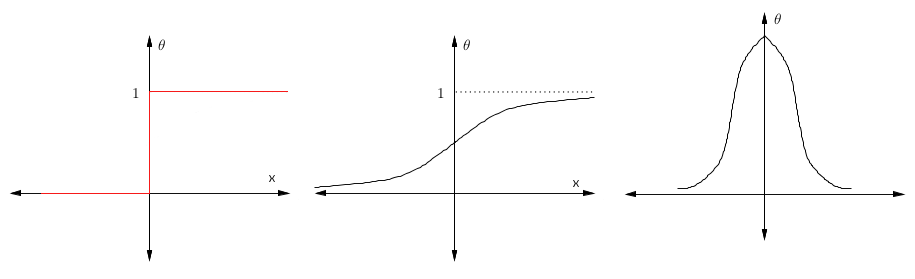
\includegraphics[width=0.6\textwidth]{activation-functions.png}
	\caption{left-most figure: $f_{w_0} (x) = \theta(wf + w...)$, $\frac{df}{dw} = 0 \rightarrow \theta$ is not a good threshold function. Using a new threshold function (center figure). Right figure: $\frac{df}{dw} = \theta\prime$.}
\end{figure}

In the visual pathway, from V1 to LGN there is a projection that is 10 times bigger then the feedfoward one. Instead of thinking about inputs and outputs, we can think about the state of the system and consider its dynamics.

\begin{figure}[H]
	\centering
	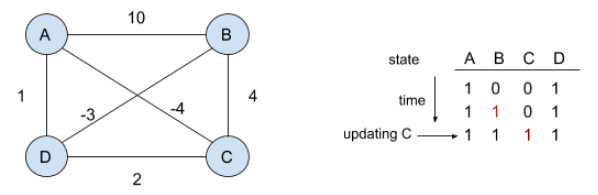
\includegraphics[width=0.8\textwidth]{gradient-descent.png}
	\label{fig:gradient-descent}
	\caption{Only one unit is updated at a time. After updating C, the network achieves a stable state, i.e., updating any unit does not change its output.}
\end{figure}

\paragraph{Asynchronous updates} 
Updating one unit at a time (in any order)
\paragraph{Synchronous updates}
Updating all units simultaneously

With asynchronous updates, a Hopfield network is guaranteed to converge.

\begin{figure}[H]
	\centering
	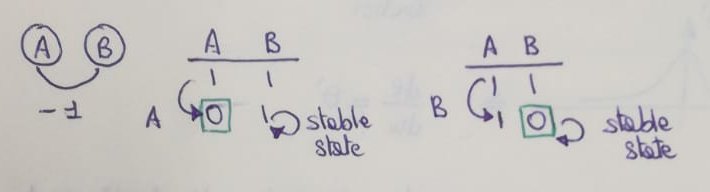
\includegraphics[width=0.6\textwidth]{convergence-asynchronous.png}
\end{figure}

Consider the sum of all weights between active units, using the model in Figure~\ref{fig:gradient-descent}. In the beggining A and D are active, the sum of the active weights is 1.

Now, we look at B and we sum the weights of the active units linked to B (D and A), see the scheme on Figure~\ref{fig:sum-weights}. The sum of active weights for B is ($10 - 3 = 7 >= 0$). If the sum $\geq 0$ we put the unit on the top part (unit active), otherwise we put the unit on the bottom (unit inactive).

If B becomes active, the sum increases (sum = 1 + 7). If B becomes inactive, the sum does not change (sum = 1).

\begin{figure}[H]
	\centering
	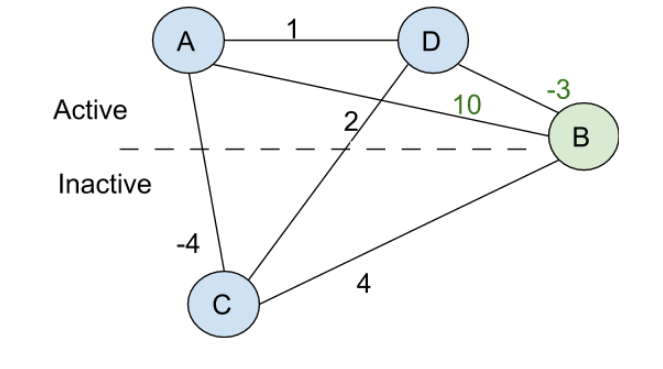
\includegraphics[width=0.5\textwidth]{sum-weights-active-units.png}
	\label{fig:sum-weights}
	\caption{Evaluation of node B}
\end{figure}

When we update a unit and change its value (active or inactive), then the sum increases or stays the same (if we are making units active). When we make units inactive, the sum doesnt change.
\end{document}
